\appendix
\setcounter{chapter}{0}
\renewcommand{\chaptername}{Appendix}
%\renewcommand{\thechapter}{\arabic{section}.\arabic{ind}}
\renewcommand{\theequation}{\Alph{chapter}.\arabic{section}.\arabic{equation}} \addcontentsline{toc}{chapter}{\numberline{}Appendix}
\setcounter{equation}{0}

\chapter{Additional Figures}
\label{first_plots}

Additional figures of spectra with \vrot $= 50,100$ \kms and \vout $= 50,75$ \kms, for all the different \tauh. 

\begin{figure}[h!]
	\begin{center}
		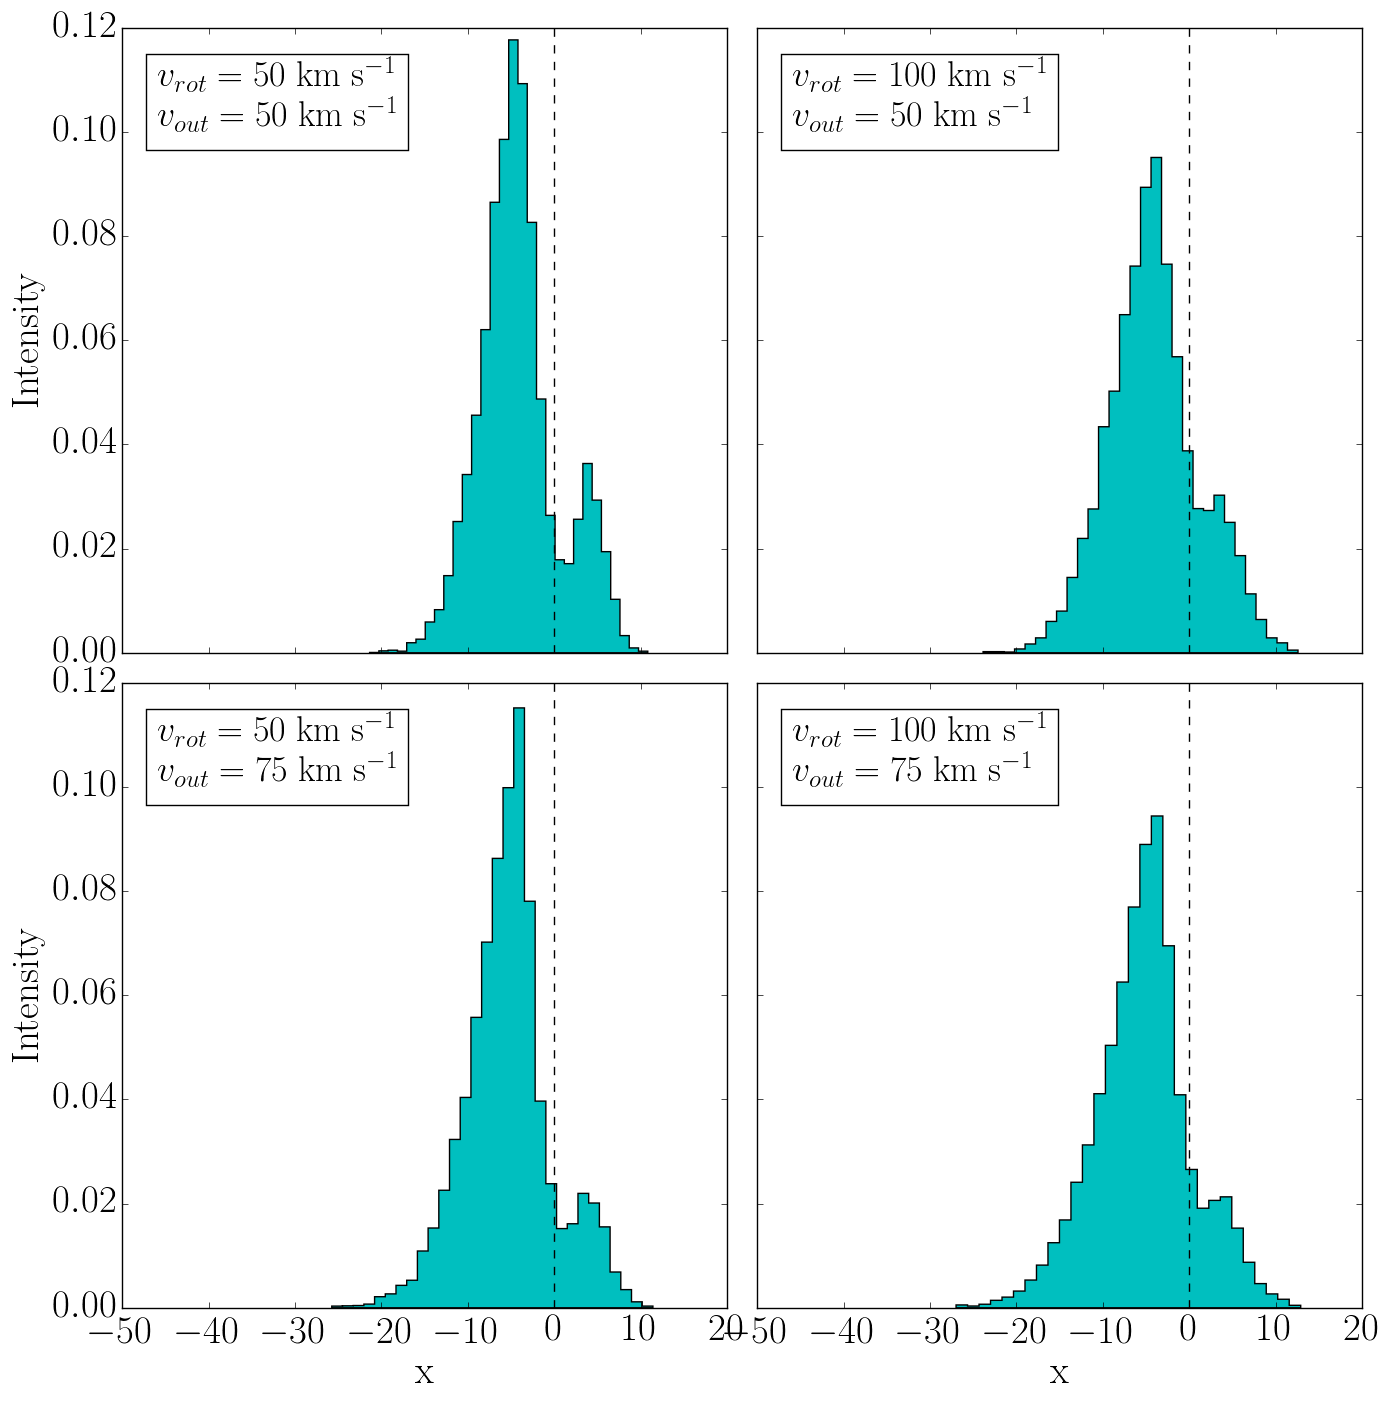
\includegraphics[width=1\textwidth]{./figures/appendix/2_tau10E5_phi83-90}
	\end{center}
	\caption{\textbf{\lya profile for \tauh$=10^5$:} With \vrot ranging $50,100$ \kms and \vout ranging $50,75$ \kms.
		\label{fig:2_tau10E5_phi83-90}}
\end{figure}

\begin{figure}[h!]
	\begin{center}
		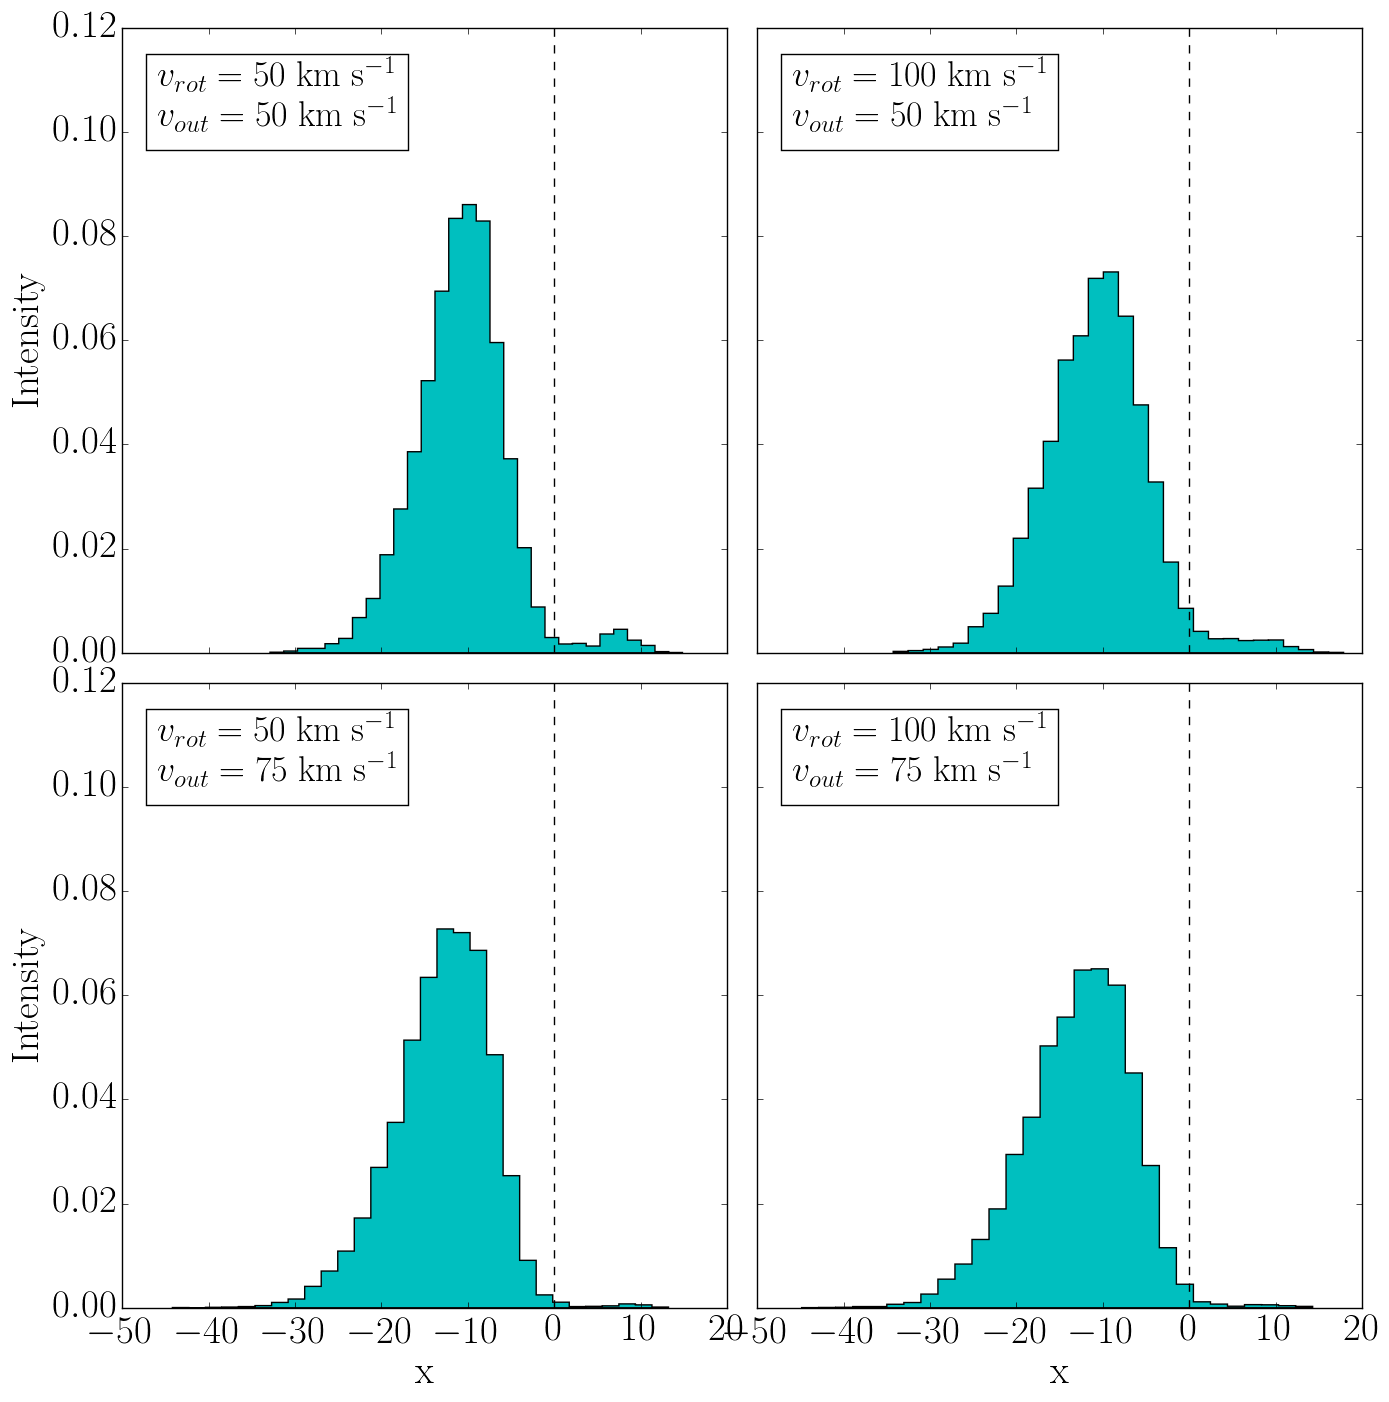
\includegraphics[width=1\textwidth]{./figures/appendix/2_tau10E6_phi83-90}
	\end{center}
	\caption{\textbf{\lya profile for \tauh$=10^6$:} With \vrot ranging $50,100$ \kms and \vout ranging $50,75$ \kms.
		\label{fig:2_tau10E6_phi83-90}}
\end{figure}

\begin{figure}[h!]
	\begin{center}
		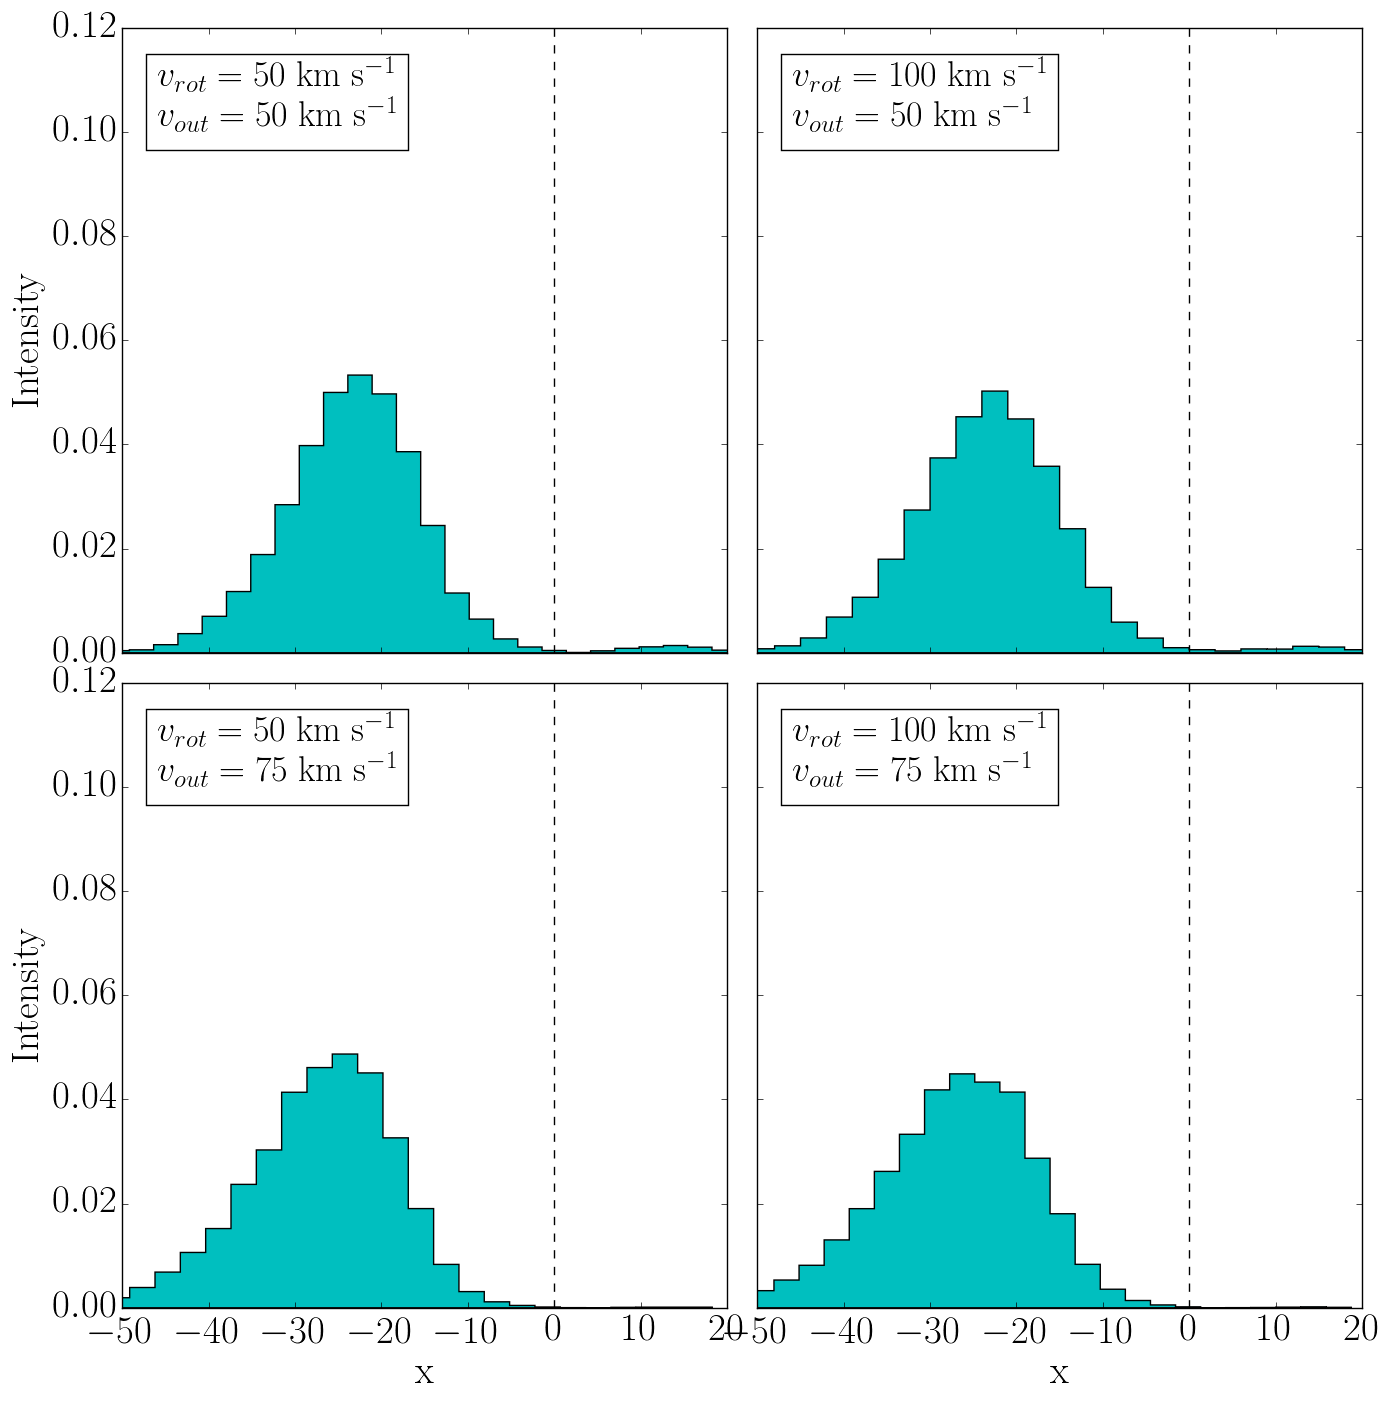
\includegraphics[width=1\textwidth]{./figures/appendix/2_tau10E7_phi83-90}
	\end{center}
	\caption{\textbf{\lya profile for \tauh$=10^7$:} With \vrot ranging $50,100$ \kms and \vout ranging $50,75$ \kms.
		\label{fig:2_tau10E7_phi83-90}}
\end{figure}